\chapter{VLAN and STP}

\section{VLAN}
By default, a device connected to a switch has level-2 connectivity to all the other devices connected to that switch.
Similarly, in a switched network, all the connected devices have layer-2 connectivity to other connected devices.

For example, Fig.~\ref{fig:No_vlan} shows a switched network that is a single layer-2 domain.

\begin{figure}
\centering
\ifpdf
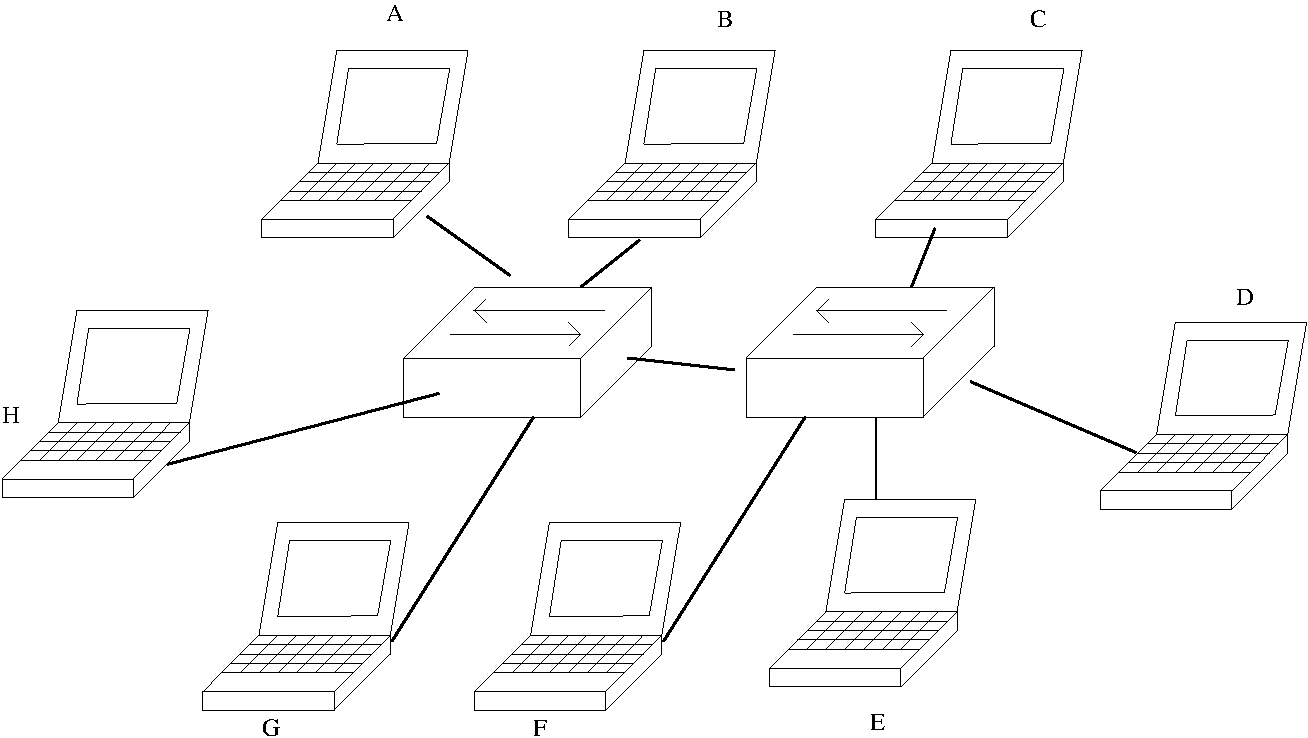
\includegraphics[width=0.5\linewidth]{Figures/No_vlan.pdf}
\else
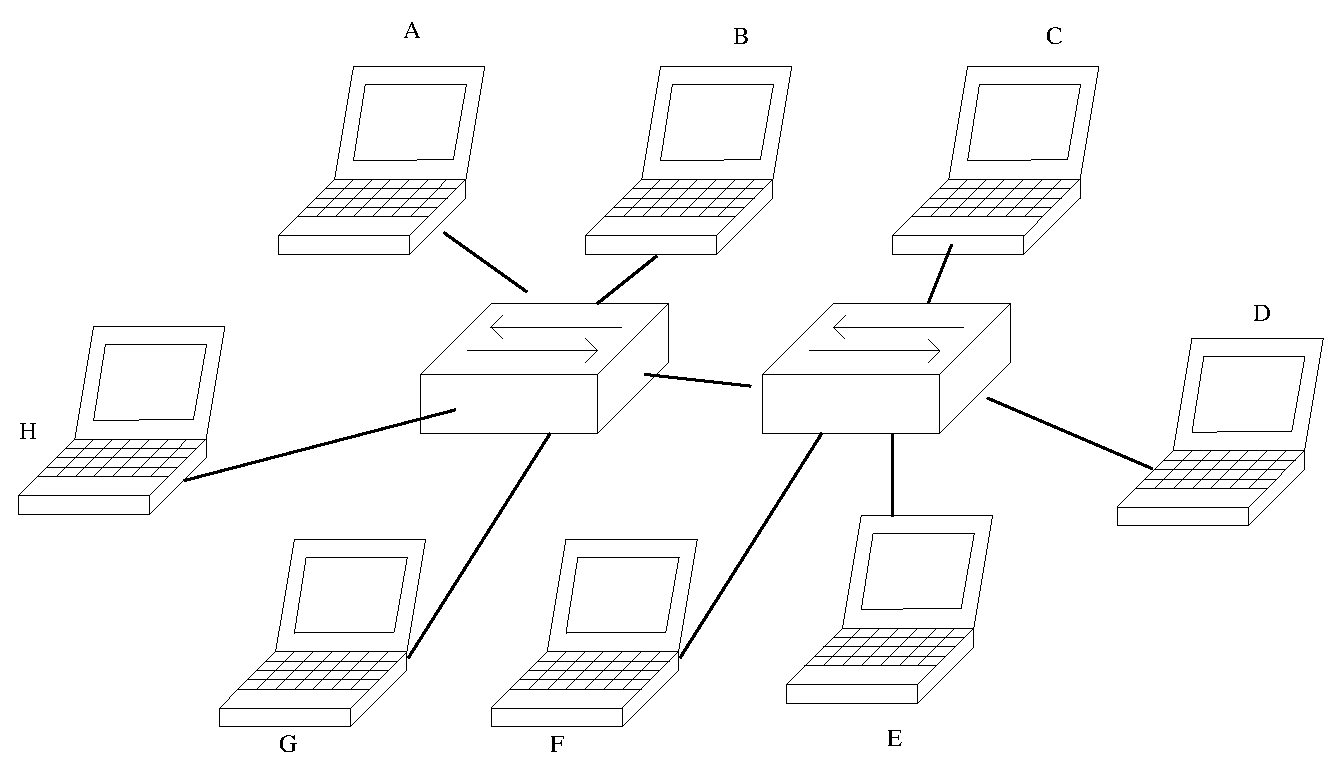
\includegraphics[width=0.5\linewidth]{Figures/No_vlan.eps}
\fi
\caption{A switched network with no VLANs.}
\label{fig:No_vlan}
\end{figure}

There are situations in which it is required to partition the network.
For example, in a campus university it might be necessary to keep wireless access points in a network separated from the servers.
If the access points are separated across multiple buildings, it would be necessary to have a switch for the access points in each building.
Similarly, if there are servers in multiple buildings, it would also be necessary to place a router in each building.
Requiring a switch for every network in every location is a solution that does not scale as the number of locations and networks increase.
It is much more convenient to have a single switch in every location and then configure the switches to keep separate link-layer networks.
This is precisely what VLANs offer.
Fig.~\ref{fig:Vlan} shows an example in which computers A, B and C are kept in a link-layer network separated from D, E and F.


\begin{figure}
\centering
\ifpdf
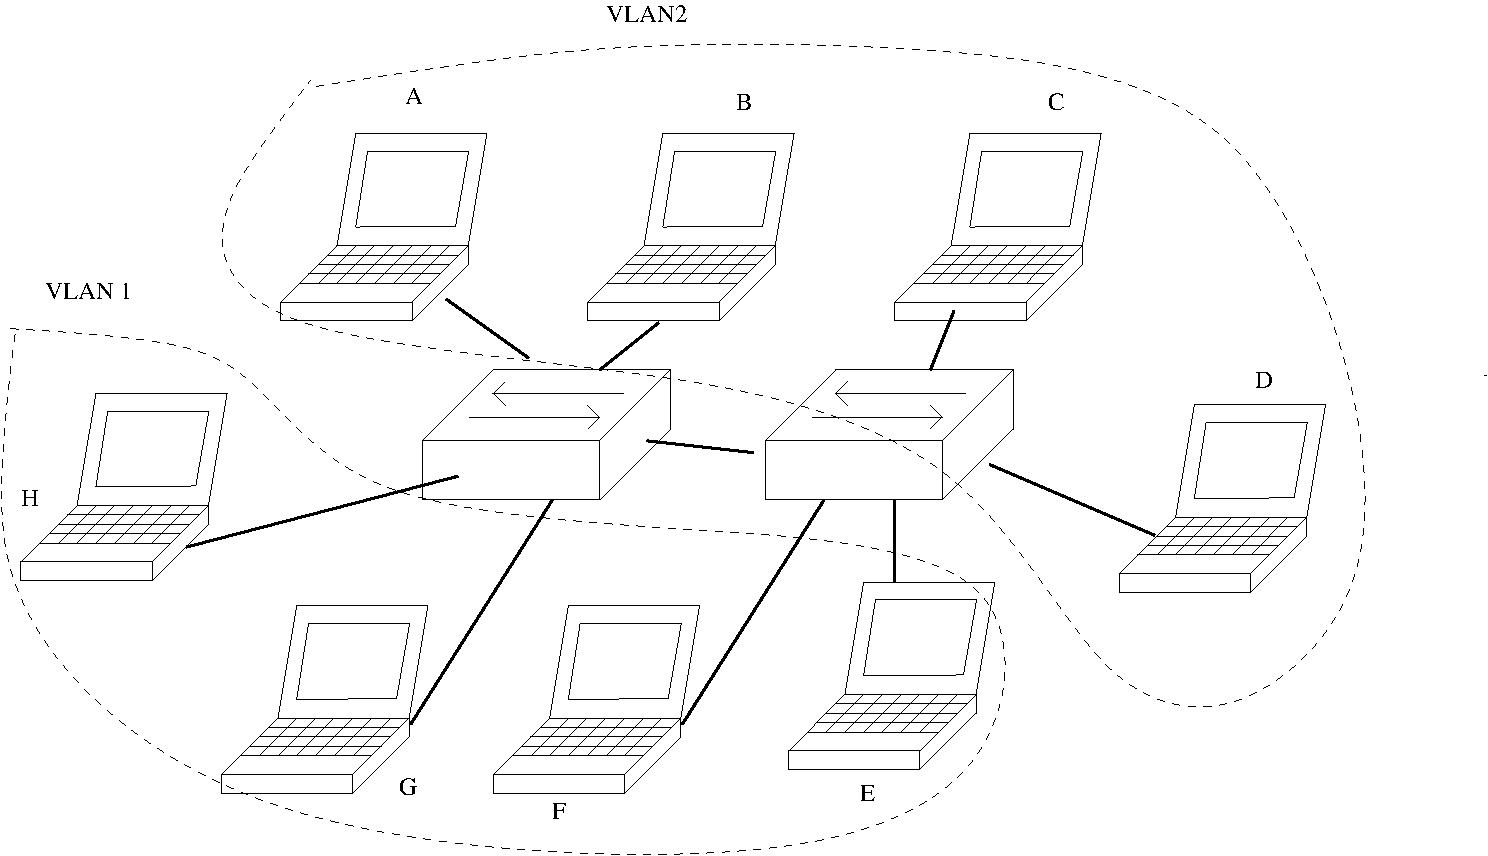
\includegraphics[width=0.5\linewidth]{Figures/Vlan.pdf}
\else
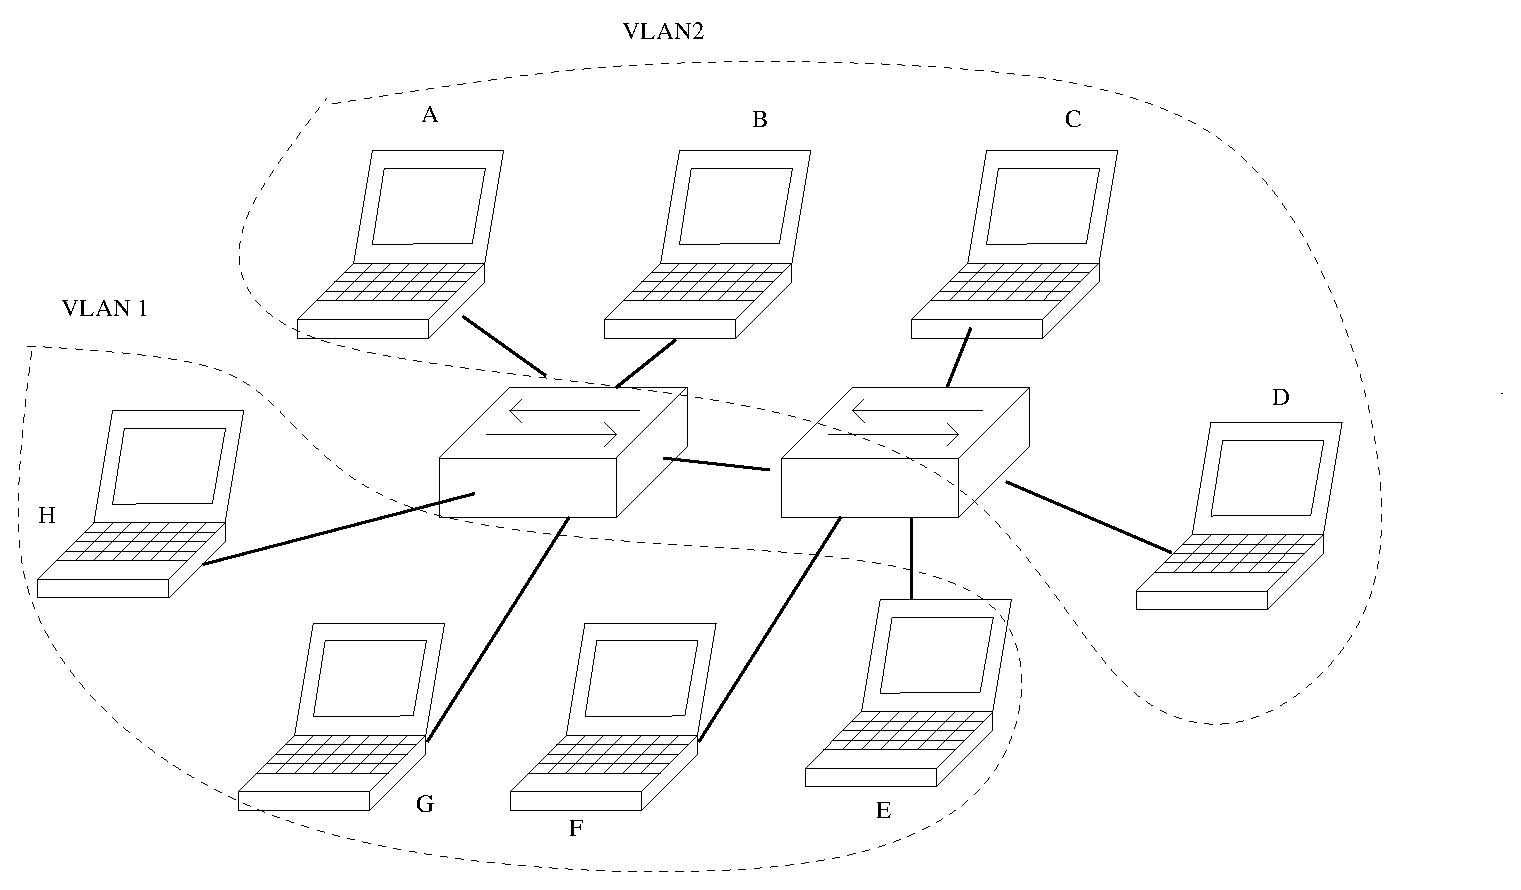
\includegraphics[width=0.5\linewidth]{Figures/Vlan.eps}
\fi
\caption{A switched network with two VLANs}
\label{fig:Vlan}
\end{figure}

VLANs are very convenient for deploying switched networks as it is possible for the network administrators to install a single switched network.
This network can later be partitioned in a flexible way simply changing the configuration of the routers.
It is possible that ethernet ports in the same room belong to different virtual lik-layer networks as it is also possible to have ethernet ports in different buildings connected to the same virtual link-layer network.

\begin{figure}
\centering
\ifpdf
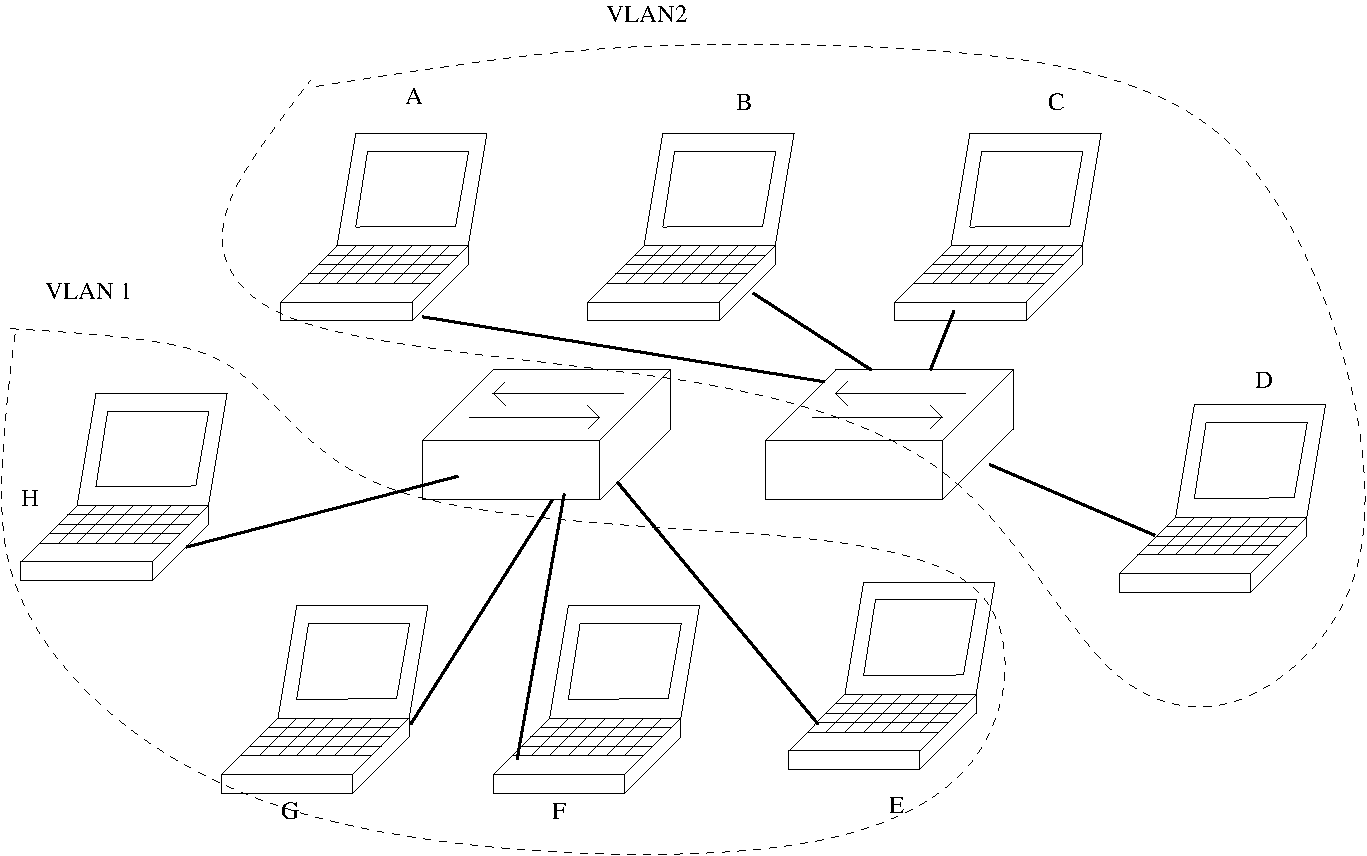
\includegraphics[width=0.5\linewidth]{Figures/Equivalent.pdf}
\else
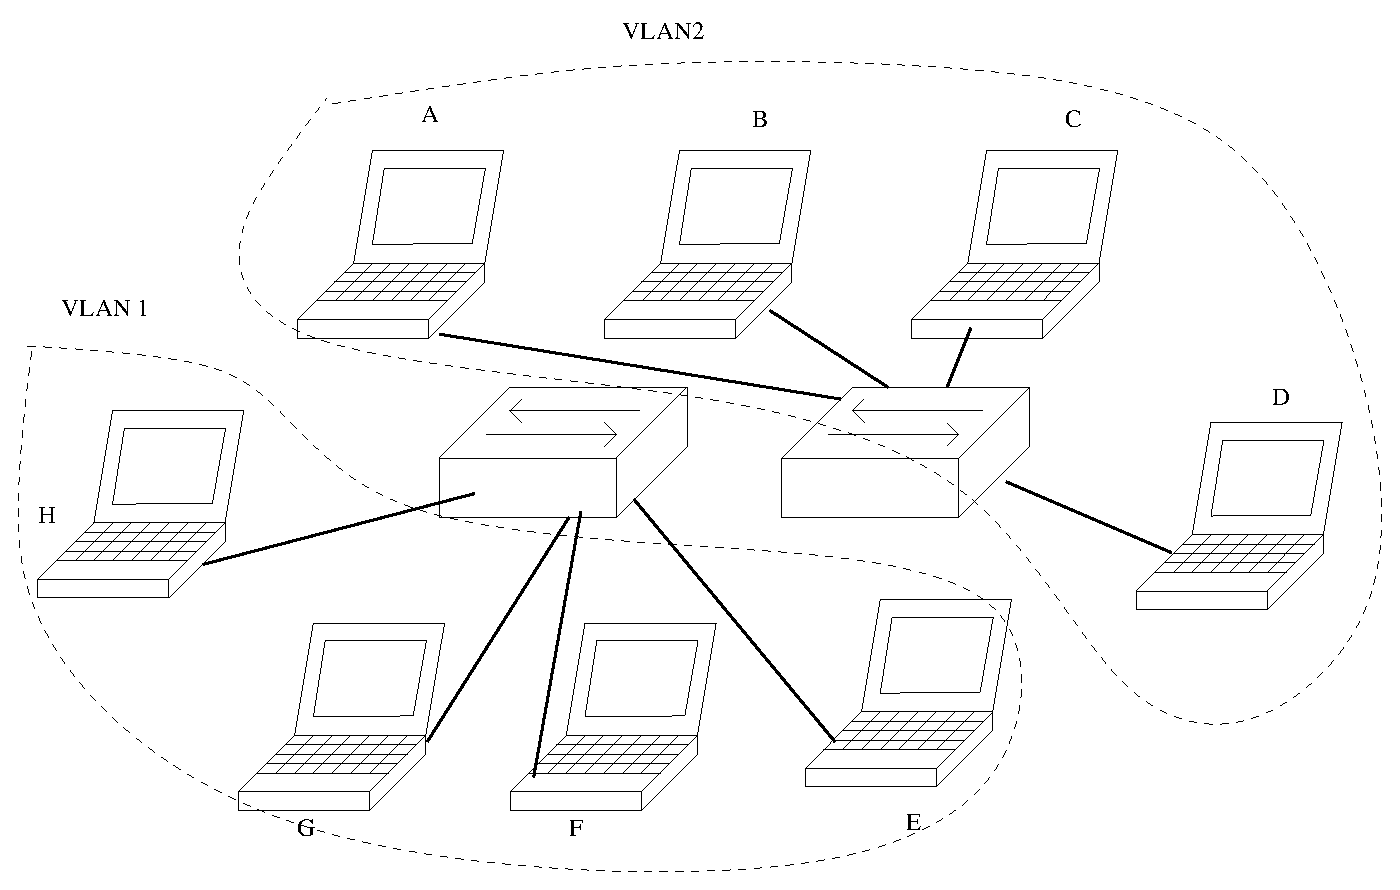
\includegraphics[width=0.5\linewidth]{Figures/Equivalent.eps}
\fi
\caption{The equivalent behaviour of the network with two VLANs depicted in Fig.~\ref{fig:Vlan}}
\label{fig:Equivalent}
\end{figure}

In a typical configuration, each VLAN contains one IP subnetwork, and it is connected to other subnetworks using a router.
Each VLAN has a number which is the VLAN identifier.
The switch ports are associated to VLAN by configuring each of the ports.  
If a switch has four ports and ports #1 and #3 are assigned to VLAN 10 while ports #2 and #4 are assigned to VLAN 20, then traffic flows from port #1 to #3 and the other way around, but it is isolated from ports #2 and #4.
This kind of assignment of a single VLAN to a port is called \emph{static-access}.

In a network deployment with multiple switches it is necessary to carry ethernet traffic from one switch to others.
One option would be to connect a separate cable for each of the existing VLANs. 
This solution is not convenient for two different reasons.
The first is that it requires many cables and many ports in each of the switches.
The second is that a new cable has to be added each time that a VLAN is created.

The alternative is to use a single cable to interconnect two routers and use that cable to transmit frames of different VLANs.
This makes the deployment and maintenance of the switched network easier.
A port carrying packets of multiple VLANs is called a trunking port.

If packets of different VLANs are transmitted over the same switch, the receiving switch needs to know to which VLAN each packet belongs to.
To this end, the sending switch will mark every frame with information about the VLAN it belongs to.



